\tikzset{>=latex} % for LaTeX arrow head

\colorlet{myred}{red!65!black}
\colorlet{mydarkblue}{blue!30!black}
\colorlet{xcol}{blue!70!black}
\colorlet{vcol}{green!70!black}
\colorlet{acol}{red!50!blue!80!black!80}
\tikzstyle{vector}=[->,very thick,xcol,line cap=round]
\tikzstyle{force}=[->,myred,thick,line cap=round]
\tikzstyle{Fproj}=[force,myred!40]
\tikzstyle{mydashed}=[dash pattern=on 2pt off 2pt]
\newcommand{\vbF}{\vb{F}}
\def\tick#1#2{\draw[thick] (#1) ++ (#2:0.1) --++ (#2-180:0.2)} %0.03*\xmax
\tikzset{
  midarr/.style={decoration={markings,mark=at position #1 with {\arrow{stealth}}},postaction={decorate}},
  midarr/.default=0.5
}

% CURVED PATH




% CLOSED PATH


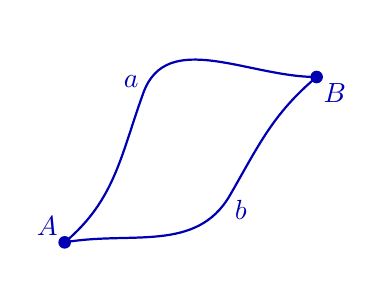
\begin{tikzpicture}
  \def\ul{0.6}
  \def\Ra{1.4}
  \def\Rb{0.8}
  \coordinate (A)  at (0,0);
  \coordinate (Ma) at (1.0,1.9);
  \coordinate (Mb) at (2.1,0.6);
  \coordinate (B)  at (3.2,2.1);
  
  % PATHS
  \draw[xcol,thick]
    (A) to[out=40,in=-110] (Ma) node[above left=-2] {$a$}
        to[out=70,in=-180] (B);
  \draw[xcol,thick]
    (A) to[out=10,in=-120] (Mb) node[below right=-2] {$b$}
        to[out=60,in=-140] (B);
  
  \fill[xcol] (A)  circle (0.08) node[above left=-1] {$A$};
  %\fill[xcol] (Ma) circle (0.08);
  %\fill[xcol] (Mb) circle (0.08);
  \fill[xcol] (B)  circle (0.08) node[below right=-1] {$B$};
  
\end{tikzpicture}
